\documentclass[11pt]{article}

% ---------------------------------------------------------------- packages
\usepackage[utf8]{inputenc}
\usepackage[T1]{fontenc}
\usepackage{lmodern}
\usepackage[margin=1in]{geometry}
\usepackage{amsmath,amssymb}
\usepackage{graphicx}
\usepackage{booktabs}
\usepackage{caption}
\usepackage{authblk}
\usepackage{xcolor}
\usepackage[round]{natbib}
\usepackage{tikz}
\usetikzlibrary{positioning,arrows.meta,shapes.geometric,fit,backgrounds,calc}
\usepackage[colorlinks=true,allcolors=blue]{hyperref}

\captionsetup{font=small,labelfont=bf}

% ---------------------------------------------------------------- metadata
\title{\bfseries Estimating Daily Sales from a Shared Behavioral Proxy:\\
Cross-Unit Temporal Disaggregation in an Affiliate-Marketing Ecosystem}

\author[1]{Parsa Hajiannejad}
\author[1]{Carlo di Bello}
\affil[1]{Universitybox}

\date{June 2026}

\begin{document}
\maketitle

% ================================================================= ABSTRACT
\begin{abstract}
\noindent
Affiliate-marketing platforms aggregate sales feeds from many partner brands,
but partners report at \emph{heterogeneous time granularities}: some deliver
transaction-level daily data, others only monthly or weekly totals. Analytics,
forecasting, and anomaly detection require a single panel at a \emph{common,
fine (daily)} granularity, yet the missing daily detail of low-frequency
reporters is unobserved. We formalize this as a \emph{cross-unit temporal
disaggregation} problem and introduce a method that recovers the daily series of
a low-frequency reporter by borrowing the within-period shape of a
high-frequency \emph{behavioral proxy} (web tracking events such as clicks and
sessions). Departing from classical disaggregation, which estimates the
indicator--target relationship within each series, we assume the
proxy-to-sales relationship is \emph{shared across brands} and learn it on
``calibration'' units that possess both true daily sales and the proxy, then
transfer it to ``target'' units that report only aggregates plus the daily
proxy. Because a per-brand intercept cancels in the disaggregation weights,
only a shared elasticity is required, so a brand with \emph{no} daily sales can
still be disaggregated while exactly conserving its reported total. On a
public, fully synthetic dataset of 60 brands over three years---calibrated to
an operational pipeline and released under a strict anonymization
protocol---a five-fold leave-units-out design recovers the shared elasticity
to within $0.3\%$ of its true value and reconstructs held-out daily sales with
$R^2=0.86$, reducing daily error by $17.6\%$ relative to the uniform split used
by naive integration pipelines. We describe the production system---behavioral
data from analytics platforms (e.g.\ GA4) joined to partner financials,
unified into one schema, and refreshed by a scheduled large-language-model
agent---and discuss when the shared-relationship assumption holds. All code and
data are released for reproducibility.
\end{abstract}

\noindent\textbf{Keywords:} temporal disaggregation; benchmarking; affiliate
marketing; behavioral proxy; transfer learning; data integration; synthetic
data; e-commerce analytics.

% ================================================================= INTRO
\section{Introduction}

Affiliate marketing is a performance-based channel in which a platform refers
users to partner merchants and is compensated per click, lead, or sale. A
platform that runs dozens of such partnerships must consolidate each partner's
sales reporting into a single analytical dataset to monitor performance,
forecast revenue, detect anomalies, and reconcile commissions. The central
operational obstacle is not volume but \emph{heterogeneity of temporal
granularity}: partners deliver data in incompatible time resolutions. In the
system that motivates this work, some partners provide transaction-level feeds
(naturally daily), while others report only a single monthly total per brand,
and a minority report weekly. Downstream consumers---time-series models,
dashboards, and daily anomaly detectors---require a \emph{common daily} panel.
For low-frequency reporters, the daily detail simply does not exist in the
source data and must be \emph{estimated}.

The naive industrial solution is to split each reported aggregate evenly across
its days (a uniform allocation). This is trivially consistent with the reported
total but discards all within-period structure: it cannot represent weekends,
promotions, paydays, or seasonal spikes, and it injects systematic error into
every daily metric built on top of it. Yet the platform almost always possesses
a second, genuinely high-frequency signal for \emph{every} brand: the
\emph{behavioral} data generated by its own tracking of user interactions
(clicks, sessions, and events recorded by web-analytics platforms). This
behavioral proxy is observed daily even for brands that report sales only
monthly. The question we address is how to use it.

We frame the task as \emph{temporal disaggregation}: recovering an unobserved
high-frequency (daily) series from an observed low-frequency aggregate using a
correlated high-frequency indicator. Classical disaggregation
\citep{ChowLin1971,Denton1971,Fernandez1981,Litterman1983} estimates the
indicator--target relationship \emph{within each series} from that series' own
aggregates. That is infeasible for a brand that has \emph{never} reported daily
sales, because there is no within-series signal from which to learn how the
proxy maps to sales. Our contribution is to relax this constraint with a
\emph{cross-unit} assumption.

\paragraph{Contributions.}
\begin{enumerate}
\item We formalize \emph{cross-unit temporal disaggregation} for affiliate
ecosystems and propose a method in which the proxy-to-sales relationship is
\emph{shared across brands}, learned on calibration units that have both true
daily sales and the proxy, and transferred to target units that report only
aggregates (Section~\ref{sec:method}). A per-brand intercept cancels in the
disaggregation weights, so only a shared elasticity is needed and aggregate
conservation is exact.
\item We position the method relative to classical disaggregation, nowcasting,
and panel/transfer-learning literatures (Section~\ref{sec:related}), and
describe an end-to-end production system that joins behavioral analytics to
partner financials and is operated by a scheduled large-language-model agent
(Section~\ref{sec:system}).
\item We release a \emph{public, fully synthetic, anonymized} dataset and a
reproducible benchmark (Section~\ref{sec:data}), and we validate the method with
a leave-units-out design that directly tests the cross-unit transfer
(Sections~\ref{sec:experiments}--\ref{sec:results}).
\end{enumerate}

% ================================================================= RELATED
\section{Related Work}\label{sec:related}

\paragraph{Temporal disaggregation and benchmarking.}
Converting a low-frequency series into a high-frequency one using a correlated
indicator is solved by a classical family of methods. \citet{ChowLin1971}
give the foundational generalized-least-squares solution, distributing
regression residuals across sub-periods under an assumed covariance structure;
\citet{Fernandez1981} and \citet{Litterman1983} extend it to non-stationary
settings via random-walk error dynamics. \citet{Denton1971} instead chooses the
high-frequency series that minimizes a quadratic movement penalty subject to the
constraint that sub-period values reproduce the observed aggregate.
\citet{DagumCholette2006} unify benchmarking, distribution, and reconciliation,
and \citet{SaxSteiner2013} provide a modern reproducible implementation. In all
of these a high-frequency indicator carries the within-period \emph{shape} while
the aggregate fixes the \emph{level}---exactly the role our behavioral proxy
plays. The distinguishing limitation is that the indicator relationship is
estimated per series.

\paragraph{Nowcasting and mixed-frequency models.}
A parallel literature uses high-frequency indicators to estimate a
not-yet-observed low-frequency target. \citet{GiannoneReichlinSmall2008}
formalize nowcasting via dynamic factor models, surveyed by
\citet{Banbura2013Nowcasting}; MIDAS regressions
\citep{GhyselsSantaClaraValkanov2006,GhyselsSinkoValkanov2007} regress a
low-frequency target on parsimonious lags of a high-frequency regressor. These
share our premise that frequent signals inform a sparse target but operate
within a single unit over time.

\paragraph{Proxy variables, pooling, and transfer.}
Our key assumption---that the proxy-to-sales mapping is shared across brands and
transferable---sits in the panel-data and hierarchical tradition.
\citet{Swamy1970} formalizes the random-coefficient regression that asks whether
slopes are common, unit-specific, or drawn from a shared distribution.
\citet{GelmanHill2006} articulate the continuum from complete pooling through
partial pooling to no pooling and show partial pooling improves predictions for
data-poor units---the regime of our target brands. \citet{PanYang2010} give the
machine-learning framing as transfer learning: knowledge learned on
label-rich source units is transferred to label-poor target units.

\paragraph{Affiliate marketing, attribution, and behavioral signals.}
\citet{EdelmanBrandi2015} establish affiliate marketing as an object of
economic study with intrinsic monitoring problems, and \citet{Berman2018} shows
how attribution rules distort incentives---motivating a unified, behaviorally
grounded dataset rather than reliance on a single reported figure.
\citet{MoeFader2004} provide foundational evidence that clickstream behavior
predicts purchase, underpinning the validity of a behavioral proxy; the
contemporary substrate for such signals is the event-based model of Google
Analytics~4 \citep{GA4Docs2023}.

\paragraph{Data integration and privacy-preserving release.}
Unifying heterogeneous feeds into one schema is the data-integration problem
formalized by \citet{Lenzerini2002}. Because we release a derived dataset, we
draw on disclosure control \citep{Hundepool2012} and differential privacy
\citep{DworkMcSherryNissimSmith2006,DworkRoth2014}, and on synthetic-data
generation and its evaluation \citep{FigueiraVaz2022,Hernandez2022}.

\paragraph{Positioning.}
Like classical disaggregation we recover a daily series from an aggregate by
borrowing shape from an indicator and we respect the aggregation constraint. We
differ in three ways: (i) the indicator relationship is \emph{transferred across
units} rather than fit per series, letting us disaggregate brands with no daily
history; (ii) the indicator is a \emph{behavioral web proxy} rather than an
economic covariate; and (iii) we contribute an automated pipeline and a
privacy-preserving public benchmark, dimensions absent from the classical
literature.

% ================================================================= METHOD
\section{Problem Formulation and Method}\label{sec:method}

\paragraph{Setup.}
Let $b \in \{1,\dots,B\}$ index brands and $t$ index days. For every brand we
observe a daily behavioral proxy $x_{b,t} \ge 0$ (e.g.\ tracking events). Brands
split into two roles. \emph{Calibration} units $\mathcal{C}$ additionally report
true daily sales $y_{b,t}$. \emph{Target} units $\mathcal{T}$ report only an
aggregate $Y_{b,P} = \sum_{t \in P} y_{b,t}$ over each reporting period $P$
(a calendar month or ISO week); their daily $y_{b,t}$ is unobserved. The goal is
to estimate $\hat{y}_{b,t}$ for $b \in \mathcal{T}$ such that the estimates
(a)~reproduce the reported aggregate, $\sum_{t\in P}\hat{y}_{b,t}=Y_{b,P}$, and
(b)~recover the within-period shape.

\paragraph{Shared proxy--sales model.}
We posit a log-log conditional mean with a brand-specific intercept and a
\emph{shared} elasticity $\beta$:
\begin{equation}
\log \mathbb{E}[y_{b,t}] \;=\; \alpha_b + \beta \, \log x_{b,t}.
\label{eq:model}
\end{equation}
The intercept $\alpha_b$ absorbs each brand's conversion level and average order
value; $\beta$ governs how daily sales scale with daily behavior and is assumed
common across brands. Equation~\eqref{eq:model} is the complete-pooling
($\beta$ shared) limit of a random-coefficient model \citep{Swamy1970}; we
return to partial pooling in Section~\ref{sec:discussion}.

\paragraph{Disaggregation weights.}
Within a period $P$, allocate the aggregate in proportion to the modeled daily
mean:
\begin{equation}
w_{b,t} \;=\; \frac{\exp(\alpha_b)\,x_{b,t}^{\beta}}
{\sum_{s\in P}\exp(\alpha_b)\,x_{b,s}^{\beta}}
\;=\; \frac{x_{b,t}^{\beta}}{\sum_{s\in P} x_{b,s}^{\beta}},
\qquad
\hat{y}_{b,t} \;=\; w_{b,t}\,Y_{b,P}.
\label{eq:weights}
\end{equation}
The brand intercept $\exp(\alpha_b)$ \emph{cancels} in the ratio. This is the
crux of the cross-unit method: estimating daily \emph{shares} requires only the
shared elasticity $\beta$, not the brand-specific level. Consequently a target
brand for which $\alpha_b$ is unidentified (no daily sales ever observed) can
still be disaggregated. By construction $\sum_{t\in P}\hat{y}_{b,t}=Y_{b,P}$, so
the benchmark constraint holds exactly. Setting $\beta=1$ recovers the
``distribute by raw clicks'' heuristic; $\beta\!\to\!0$ recovers the uniform
split. The same weights disaggregate the monetary total $Y^{\$}_{b,P}$.

\paragraph{Estimating the shared elasticity.}
We estimate $\beta$ on calibration units only, using a within (fixed-effects)
estimator that absorbs $\alpha_b$. With $\tilde{u}_{b,t}=\log x_{b,t} -
\overline{\log x_{b,\cdot}}$ and $\tilde{v}_{b,t}=\log y_{b,t} -
\overline{\log y_{b,\cdot}}$ the brand-demeaned logs,
\begin{equation}
\hat{\beta} \;=\;
\frac{\sum_{b\in\mathcal{C}}\sum_{t}\tilde{u}_{b,t}\,\tilde{v}_{b,t}}
{\sum_{b\in\mathcal{C}}\sum_{t}\tilde{u}_{b,t}^{2}}.
\label{eq:beta}
\end{equation}
Demeaning makes $\hat{\beta}$ invariant to each brand's level, so the estimand
is precisely the transferable quantity in Eq.~\eqref{eq:weights}. Estimating
$\beta$ on a held-out set of brands and applying it to others is a direct test
of the shared-relationship assumption.

% ================================================================= SYSTEM
\section{The E-commerce Case-Study System}\label{sec:system}

The method is deployed in a production affiliate platform. Two data families are
joined (Figure~\ref{fig:pipeline}). \emph{Behavioral} data---page views,
clicks, and conversion events---are collected by web-analytics tooling (e.g.\
the event-based model of GA4, \citealp{GA4Docs2023}) and aggregated to a daily
proxy $x_{b,t}$ per brand. \emph{Financial} data---units sold and revenue---are
delivered directly by each partner in the partner's own spreadsheet format and
native granularity. A schema-unification layer \citep{Lenzerini2002} maps every
partner feed onto one global schema keyed by (brand, date, event type), parsing
each partner's idiosyncratic columns into a common representation. Low-frequency
financial feeds are then disaggregated to daily via Eq.~\eqref{eq:weights} using
the behavioral proxy, and the unified daily panel is written to a cloud
warehouse with an idempotent, delete-then-load upsert that makes re-runs safe.

Orchestration is fully automated by a scheduled large-language-model agent
(an Anthropic Claude agent) that runs nightly: it refreshes the partner sources,
invokes the parsers and the disaggregation, performs the warehouse load, and
emits a reconciliation report. This replaces brittle, hand-run scripts with a
single scheduled task and provides a natural-language audit trail of each run.

\begin{figure}[t]
\centering
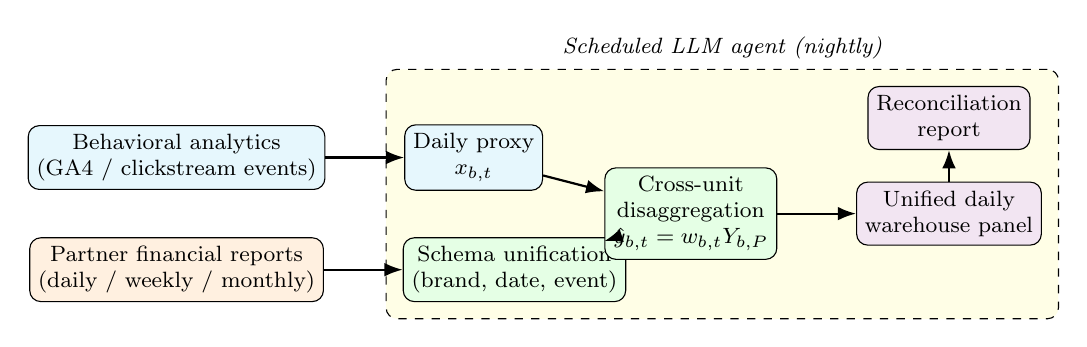
\begin{tikzpicture}[
  font=\footnotesize,
  node distance=6mm and 10mm,
  box/.style={draw,rounded corners,align=center,minimum height=8mm,
              inner sep=3pt,fill=blue!5},
  beh/.style={box,fill=cyan!10},
  fin/.style={box,fill=orange!12},
  core/.style={box,fill=green!10},
  snk/.style={box,fill=violet!10},
  ar/.style={-{Latex[]},thick}
]
% sources
\node[beh] (ga) {Behavioral analytics\\(GA4 / clickstream events)};
\node[fin,below=of ga] (fin) {Partner financial reports\\(daily / weekly / monthly)};
% proxy + unify
\node[beh,right=of ga] (proxy) {Daily proxy\\$x_{b,t}$};
\node[core,right=of fin] (unify) {Schema unification\\(brand, date, event)};
% method
\node[core,right=14mm of $(proxy)!0.5!(unify)$] (disagg)
   {Cross-unit\\disaggregation\\$\hat y_{b,t}=w_{b,t}Y_{b,P}$};
% warehouse + outputs
\node[snk,right=of disagg] (wh) {Unified daily\\warehouse panel};
\node[snk,above=4mm of wh] (rec) {Reconciliation\\report};
% agent band
\begin{scope}[on background layer]
\node[draw,dashed,rounded corners,fill=yellow!10,inner sep=6pt,
      fit=(proxy)(unify)(disagg)(wh)(rec),label=above:{\itshape Scheduled LLM agent (nightly)}] {};
\end{scope}
\draw[ar] (ga) -- (proxy);
\draw[ar] (fin) -- (unify);
\draw[ar] (proxy) -- (disagg);
\draw[ar] (unify) -- (disagg);
\draw[ar] (disagg) -- (wh);
\draw[ar] (wh) -- (rec);
\end{tikzpicture}
\caption{Production pipeline. Behavioral analytics yield a daily proxy for every
brand; heterogeneous partner financial feeds are unified onto one schema;
low-frequency feeds are disaggregated to daily using the shared-elasticity
weights (Eq.~\ref{eq:weights}); the unified panel is loaded to the warehouse.
The shaded band is orchestrated nightly by a scheduled large-language-model
agent.}
\label{fig:pipeline}
\end{figure}

% ================================================================= DATA
\section{Data and Anonymization}\label{sec:data}

\paragraph{Why synthetic.}
The operational data contain commercially sensitive partner sales and would
expose the platform and its partners to legal and contractual risk if released.
We therefore release a \emph{fully synthetic} dataset that reproduces the
\emph{structure} required to study the method---the proxy-to-sales relationship,
weekly and annual seasonality, and cross-brand magnitude heterogeneity---without
reproducing any real value or identity. This follows established practice in
privacy-preserving data publishing \citep{Hundepool2012,FigueiraVaz2022,
Hernandez2022}.

\paragraph{Anonymization protocol.}
(i)~Brands are labelled with neutral codes (\texttt{BR-001}\,\dots) and a
generic sector tag; no real partner name appears. (ii)~Every numeric value is a
fresh pseudo-random draw, not a transformed real record, so no released figure
coincides with any real figure; a per-brand secret multiplicative factor further
decouples magnitudes. (iii)~The generator is seeded and published, so the
dataset is exactly reproducible while remaining non-identifying. Because the
release contains no real microdata, re-identification is not possible by
construction.

\paragraph{Data-generating process.}
For brand $b$ on day $t$ the proxy is
$x_{b,t}\sim\mathrm{Poisson}\!\big(\ell_b\,W(t)\,A(t)\,G(t)\big)$, where
$\ell_b$ is a brand level drawn across roughly two orders of magnitude, $W$ is a
weekly profile (weekday peak, weekend dip), $A$ an annual profile (spring/summer
and a late-November promotional peak), and $G$ a mild growth trend. Daily sales
follow Eq.~\eqref{eq:model} with a brand-specific intercept and a per-brand
slope $\beta_b=\beta+\varepsilon_b$, $\varepsilon_b\sim\mathcal{N}(0,s_\beta^2)$,
times multiplicative lognormal noise. We set the shared elasticity $\beta=0.88$
and $s_\beta=0.05$, so the shared-relationship assumption holds only
\emph{approximately}---a deliberate stress test. Monetary value is units times a
brand average order value.

\paragraph{Released files.}
The dataset spans 60 brands over 1{,}096 days (2023--2025):
\texttt{behavioral\_proxy\_daily.csv} (65{,}760 rows, all brands);
\texttt{sales\_calibration\_daily.csv} (24{,}112 rows, the 22 calibration
brands' true daily sales); \texttt{sales\_target\_aggregate.csv} (2{,}832 rows,
the 38 target brands' monthly/weekly totals); and \texttt{brand\_registry.csv}.
Table~\ref{tab:data} summarizes the composition.

\begin{table}[t]
\centering
\caption{Composition of the released synthetic dataset.}
\label{tab:data}
\begin{tabular}{lccc}
\toprule
Role & Reporting granularity & \# Brands & Daily sales released? \\
\midrule
Calibration & daily (transactional) & 22 & yes (ground truth) \\
Target & monthly & 26 & no (aggregate only) \\
Target & weekly & 12 & no (aggregate only) \\
\midrule
\multicolumn{2}{l}{Total} & 60 & \\
\bottomrule
\end{tabular}
\end{table}

Figure~\ref{fig:problem} illustrates the core difficulty for one target brand:
the behavioral proxy is observed every day, whereas sales are reported as a
single total per month.

\begin{figure}[t]
\centering
\includegraphics[width=0.92\linewidth]{figures/fig1_granularity_problem.pdf}
\caption{The granularity mismatch for a representative target brand. The
high-frequency behavioral proxy (blue) is available daily; reported sales exist
only as twelve monthly totals (shaded bands), so the daily sales shape is
unobserved and must be estimated.}
\label{fig:problem}
\end{figure}

% ================================================================= EXPERIMENTS
\section{Experimental Design}\label{sec:experiments}

We evaluate the central claim---that the proxy-to-sales relationship transfers
across brands---with a \emph{five-fold leave-units-out} protocol. The 22
calibration brands are partitioned into five folds. In each fold, $\hat{\beta}$
is estimated (Eq.~\ref{eq:beta}) on the brands \emph{outside} the fold; the
held-out brands are then treated as pseudo-targets: their true daily sales are
aggregated to monthly totals, the daily series is reconstructed from those
totals using the transferred $\hat{\beta}$ (Eq.~\ref{eq:weights}), and the
reconstruction is compared against the known daily truth. Because $\hat\beta$
never sees the held-out brands, this measures genuine cross-unit transfer.

\paragraph{Baselines.} (i)~\textsc{Uniform}: split each total equally across its
days ($\beta\!=\!0$), the standard industrial heuristic. (ii)~\textsc{Proxy
linear}: weight by raw proxy ($\beta\!=\!1$). (iii)~\textsc{Proxy power}: our
method with estimated $\hat{\beta}$.

\paragraph{Metrics.} We report the symmetric mean absolute percentage error
(sMAPE) and mean absolute error (MAE) between estimated and true daily sales,
the coefficient of determination $R^2$ on daily values, and the aggregate
conservation error $|\sum_t\hat{y}_{b,t}-Y_{b,P}|$. Metrics are averaged over
the five folds (mean\,$\pm$\,s.d.). We additionally sweep the true elasticity
$\beta\in[0.3,1.7]$ in an independent simulation to quantify the value of
estimating $\beta$ rather than fixing it.

% ================================================================= RESULTS
\section{Results}\label{sec:results}

\paragraph{The shared elasticity is recovered and transfers.}
The full-sample within estimator gives $\hat{\beta}=0.882$, within $0.3\%$ of
the true shared value $0.88$. Per-brand elasticities are tightly concentrated
(mean $0.883$, s.d.\ $0.052$; Figure~\ref{fig:beta}), matching the injected
slack $s_\beta=0.05$ and confirming that a single shared slope is a good
approximation for this population.

\begin{figure}[t]
\centering
\includegraphics[width=0.55\linewidth]{figures/fig2_beta_recovery.pdf}
\caption{Distribution of per-brand estimated elasticities $\hat{\beta}_b$ across
calibration brands. The mean of the per-brand estimates (green) coincides with
the true shared value (orange dashed), supporting the shared-relationship
assumption.}
\label{fig:beta}
\end{figure}

\paragraph{Held-out daily reconstruction is accurate.}
Table~\ref{tab:results} reports the leave-units-out results. Using only the
transferred elasticity, the proxy method reconstructs held-out daily sales with
$R^2=0.86$ on average and sMAPE $14.1\%$, versus $R^2=0.80$ and sMAPE $17.1\%$
for the uniform split---a $17.6\%$ relative reduction in daily error from a
signal the platform already collects. Aggregate conservation error is zero to
numerical precision for all methods, as guaranteed by Eq.~\eqref{eq:weights}.
Figure~\ref{fig:results}A--C shows the held-out fit, the method comparison, and
within-month shape recovery for an example brand, where the uniform baseline is
flat by construction while the proxy method tracks the true daily profile.

\begin{table}[t]
\centering
\caption{Daily reconstruction accuracy under five-fold leave-units-out
(mean\,$\pm$\,s.d.\ over folds). Lower is better for sMAPE/MAE; higher for
$R^2$. The proxy methods use only the elasticity transferred from other brands.}
\label{tab:results}
\begin{tabular}{lccc}
\toprule
Method & sMAPE (\%) & MAE (units) & $R^2$ \\
\midrule
Uniform ($\beta=0$)              & $17.10 \pm 0.29$ & $6.70 \pm 0.16$ & $0.802 \pm 0.135$ \\
Proxy linear ($\beta=1$)         & $14.13 \pm 0.25$ & $5.59 \pm 0.13$ & $0.858 \pm 0.094$ \\
Proxy power ($\hat{\beta}$, ours)& $\mathbf{14.09 \pm 0.24}$ & $\mathbf{5.58 \pm 0.13}$ & $\mathbf{0.859 \pm 0.093}$ \\
\bottomrule
\end{tabular}
\end{table}

\paragraph{When does estimating $\beta$ matter?}
On this population $\hat{\beta}=0.88$ is close to $1$, so \textsc{proxy power}
only marginally beats \textsc{proxy linear} ($14.09$ vs $14.13$)---a difference
well within fold-to-fold variability and not, on its own, statistically
meaningful here. The sweep in
Figure~\ref{fig:results}D explains why and when the elasticity matters:
\textsc{proxy power} attains the lowest error across the \emph{entire} range of
true $\beta$, whereas \textsc{proxy linear} degrades as the true elasticity
departs from $1$, and \textsc{uniform} is worst throughout and collapses when
$\beta$ is small. Estimating $\beta$ is therefore a robustness guarantee: it
costs nothing when $\beta\approx1$ and protects against substantial error when
the proxy-to-sales relationship is strongly concave or convex.

\begin{figure}[t]
\centering
\includegraphics[width=\linewidth]{figures/fig3_results.pdf}
\caption{(\textbf{A})~Held-out true vs.\ estimated daily sales for the proxy
method (one fold). (\textbf{B})~Daily reconstruction error by method (five-fold
leave-units-out; error bars are s.d.\ across folds). (\textbf{C})~Within-month
shape recovery for an example held-out brand: the proxy method tracks the true
daily profile while the uniform split is flat. (\textbf{D})~Sensitivity sweep:
the estimated-elasticity method is best across all true $\beta$, justifying
estimation over fixed weights.}
\label{fig:results}
\end{figure}

\paragraph{Application to true target brands.}
Applying the full-sample $\hat{\beta}$ to all 38 target brands produces a
complete daily panel whose per-brand totals reproduce the reported aggregates to
within $9\times10^{-5}\%$ (rounding only), confirming that the integration is
both fine-grained and exactly reconciled.

% ================================================================= DISCUSSION
\section{Discussion}\label{sec:discussion}

\paragraph{Interpretation.}
The behavioral proxy converts an unobserved daily quantity into an accurately
estimable one. The practical gain over the uniform split---used by many naive
integration pipelines---is large and free, since the proxy is already collected.
The more conceptually important result is that the proxy-to-sales \emph{shape}
is governed by an elasticity that is stable across brands and can be borrowed
from brands that do have daily data, enabling disaggregation of brands that
never will.

\paragraph{Relation to classical disaggregation.}
Equation~\eqref{eq:weights} is a Chow--Lin/Denton-style benchmark in which the
indicator is a behavioral proxy and the indicator coefficient is
\emph{transferred across units} rather than fit per series. This is the key
departure: classical estimators require each series' own aggregates to learn its
indicator relationship, whereas the shared-elasticity assumption supplies that
relationship externally. Our leave-units-out validation is, in effect, an
empirical test of whether that external relationship is valid.

\paragraph{When the assumption holds.}
Complete pooling (one shared $\beta$) is justified when brands share a conversion
mechanism, as in a single platform whose proxy is measured consistently across
partners. When brands differ systematically---distinct product categories,
price points, or audiences---the principled relaxation is a random-coefficient
or hierarchical model \citep{Swamy1970,GelmanHill2006} with partial pooling, in
which $\beta_b$ is shrunk toward a population mean; data-rich brands inform their
own slope while data-poor brands borrow strength. Our framework accommodates
this directly by replacing the shared $\hat\beta$ in Eq.~\eqref{eq:weights} with
a brand-specific posterior slope. Sector- or category-level pooling is a natural
middle ground. For the present population, the narrow spread of per-brand
estimates (s.d.\ $0.052$ around a mean of $0.883$) is consistent with complete
pooling; a formal poolability test of slope homogeneity \citep{Swamy1970} is a
natural confirmatory step we leave to future work.

% ================================================================= LIMITATIONS
\section{Limitations}\label{sec:limitations}

First, disaggregated daily values are \emph{estimates}, not measurements;
validation conserves and reconstructs aggregates but cannot certify any single
day for a true target brand, which by definition lacks ground truth. Daily
figures should be labelled as modeled. Second, the method assumes the proxy is
informative and available for all brands and that its measurement is comparable
across brands; a brand whose proxy is mismeasured or whose conversion is
proxy-independent will be poorly served. Third, our evidence is on synthetic
data calibrated to one operational system; while the generating process embeds
realistic structure and an honest assumption-violation ($s_\beta>0$), external
validity to other ecosystems should be confirmed on their own calibration units.
Fourth, the shared-elasticity model is intentionally simple; richer
specifications (lagged proxy effects, promotion indicators, hierarchical
slopes) are natural extensions.

% ================================================================= ETHICS
\section{Ethical, Legal, and Privacy Considerations}\label{sec:ethics}

The behavioral data underlying the proxy derive from user web interactions and
must be collected and processed under applicable privacy law and platform
policy; in this work the proxy is used only in aggregate daily counts per brand,
never at the individual-user level. The released dataset contains no personal
data and no real commercial figures: it is fully synthetic, with coded brand
identifiers, freshly drawn and rescaled values, and a seeded, published
generator (Section~\ref{sec:data}). This design eliminates re-identification and
commercial-confidentiality risk while preserving reproducibility, consistent
with disclosure-control and synthetic-data guidance
\citep{Hundepool2012,FigueiraVaz2022}. No real partner is identified or
identifiable from any released artifact.

% ================================================================= CONCLUSION
\section{Conclusion}\label{sec:conclusion}

We introduced cross-unit temporal disaggregation for affiliate-marketing
ecosystems: a method that estimates the daily sales of low-frequency reporters
by transferring a shared behavioral-proxy elasticity learned from brands with
daily data, while exactly conserving reported aggregates. The approach unifies
heterogeneous partner feeds into a single daily panel, is deployed in a
production pipeline orchestrated by a scheduled large-language-model agent, and
on a public synthetic benchmark recovers the shared elasticity to within $0.3\%$
and reconstructs held-out daily sales at $R^2=0.86$, cutting daily error by
$17.6\%$ over the uniform split. The estimated elasticity provides robustness
across the full range of proxy-to-sales relationships. Future work includes
hierarchical (partial-pooling) elasticities, richer behavioral covariates, and
validation across multiple ecosystems.

% ================================================================= STATEMENTS
\section*{Data and Code Availability}
All code (data generator, estimation, experiments, and figure scripts) and the
fully synthetic dataset are released at
\url{https://github.com/Parsa-Hajian/affiliate-granularity-proxy}.
The dataset is reproducible from the published seed.

\section*{Author Contributions}
P.H.\ designed the method, implemented the system and experiments, and drafted
the manuscript. C.d.B.\ contributed to the problem formulation, validation
design, and manuscript revision.

\section*{Conflicts of Interest}
The authors are affiliated with the platform that motivated this study. No real
commercial data are disclosed.

\bibliographystyle{plainnat}
\bibliography{refs}

\end{document}
